\chapter{Appendix}
\label{sec:App} 

\section{Glossary}


\begin{table}[H]
\centering
\label{my-label}
\begin{tabular}{|c|l|}
\hline
\textbf{Blog}      & Abbreviation to WebLog                                                                                                            \\ \hline
\textbf{Emoticon}  & Short for emotion icon. e.g. ":D", ":)", ":-)"                                                                                    \\ \hline
\textbf{Hashtag}   & Topic labels used in Twitter posts.                                                                                               \\ \hline
\textbf{Microblog} & \begin{tabular}[c]{@{}l@{}}Sites where users express their ideas in the form of\\ small units of text. e.g. Twitter.\end{tabular} \\ \hline
\textbf{Tweet}     & Short message or post.                                                                                                            \\ \hline
\textbf{SO}        & Sentiment Orientation                                                                                                             \\ \hline
\textbf{NLP}       & natural language processing                                                                                                       \\ \hline
\textbf{Lexicon}   & Dicctionary or lexical resource                                                                                                   \\ \hline
\end{tabular}
\end{table}

\clearpage

\section{Technical Specifications}

The source code of the project can be downloaded from the following link which points to
the Git repository of the EIS group, University of Bonn. 

\textbf{Link to thesis repository: }

https://github.com/EIS-Bonn/Theses/tree/master/2015/Cristobal\_Leiva

To run the application, the system has to fulfill the following requirements and the user
needs to follow the instructions given below.

\textbf{Requirements:}

\begin{itemize} 
\itemsep0em  

\item Node.js + NPM

\item Latest MongoDB

\item Bower (get by running "npm install -g bower")

\item Gulp (get by running "npm install -g gulp")


\end{itemize}

\textbf{How to Install:}

\begin{enumerate} 
\itemsep0em  

\item Install the required NodeJS modules: npm install

\item Configure Twitter API keys: pen config.sample.js and fill in the required keys under the twitter app
config and save it as config.js

\item To start NodeJS server: start mongo then run the command "gulp"

\item Run the web browser: http://localhost:8082/resa


\end{enumerate}

\clearpage
\section{SentiTrack GUI}

\begin{figure}[H]
    \centering
    \caption{SentiTrack front-end, bubble cloud}
    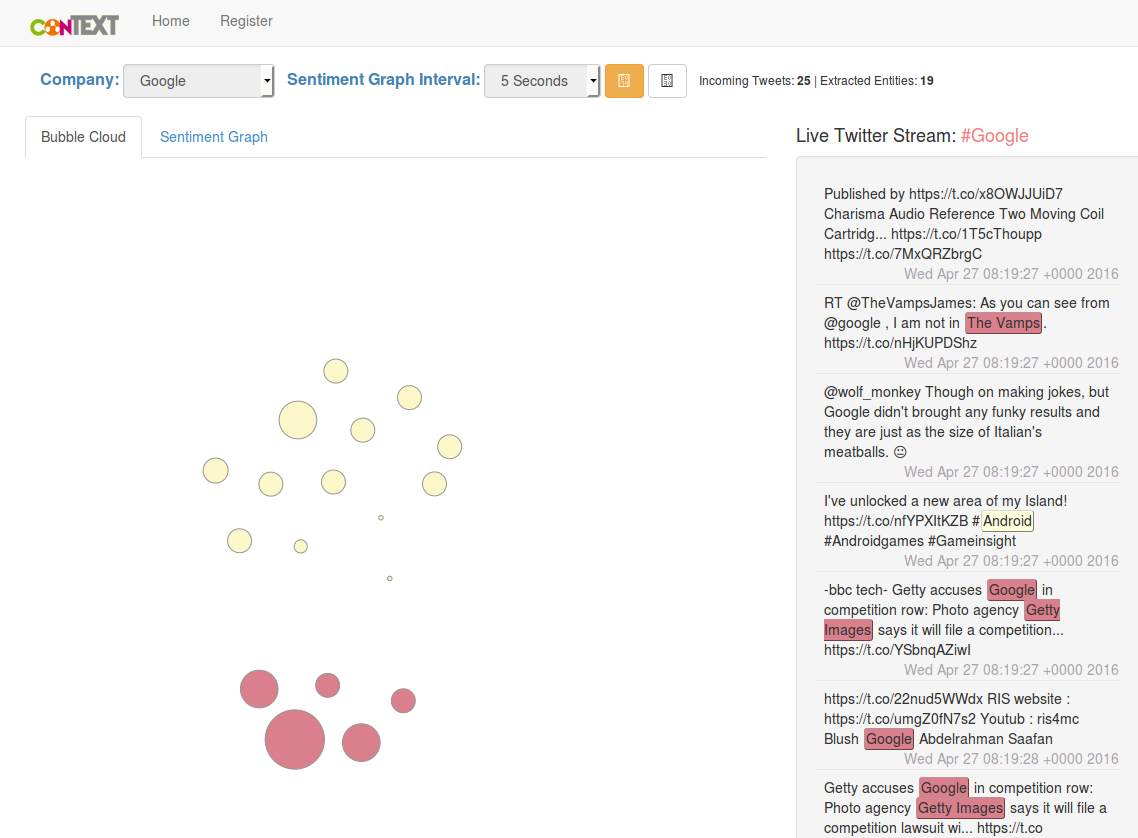
\includegraphics[width=\linewidth]{19_sentitrack_01}
    \label{}
\end{figure}

\begin{figure}[H]
    \centering
    \caption{SentiTrack front-end, live sentiment data}
    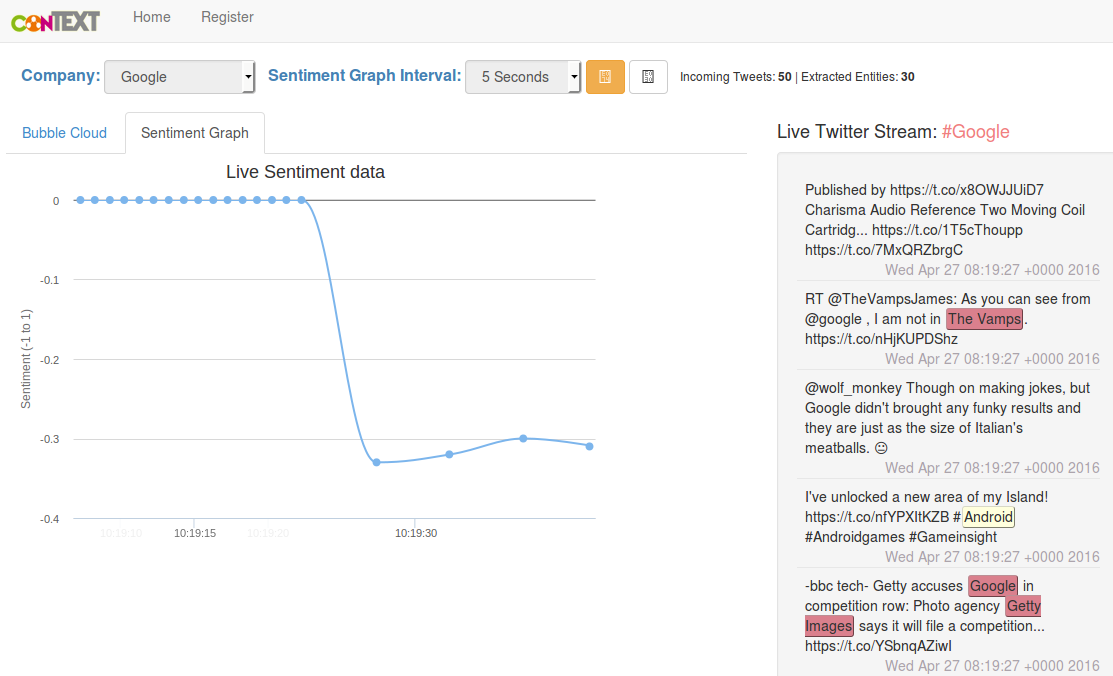
\includegraphics[width=\linewidth]{20_sentitrack_02}
    \label{}
\end{figure}
